\documentclass[12pt]{article}
\parindent0pt
\usepackage{ctex}
\usepackage{amsmath}
\usepackage{mathtools,amssymb}
\usepackage[utf8]{inputenc}
\usepackage{tikz}
\usetikzlibrary{automata,positioning,arrows}
\title{CS 2AC3 Assignment 4}
\author{Longyu Zhu}
\begin{document}
\section*{1.Which of the followings are a CFL? 
For CFLs provide a CFG in Chomoskey normal form 
(no need to prove the equivalance); if a language in not CFL then prove your answer (e.g., using pumping lemma for CFLs).}
\subsection*{ $\left(a\right) \left\{a^m b^n c^p | m,n,p\geq 0,m\neq n~and~n\neq p\right\}$ }
at the first, assume m=3,n=2,p=4 that will meet the condition of quetsion say, and then asumme $z\in \left(a\right)~ and ~z=\{aaabbcccc\}$ 
thus z=uvwxy, $v,x\neq\varepsilon$ and $|vwk|\leq k\left(length~of~z=2+3+4=9\right)$\\
$u,v,w,x,y\in z\Rightarrow u=\{aa\},~v=\{a\} ,~w=\{b\},~ x=\{b\}, ~y=\{cccc\}$\\
At the first $v,x\neq \varepsilon\Rightarrow v=\{a\}\neq \varepsilon~and~x=\{b\}\neq\varepsilon$ that is true.\\
and then $|vwx|\leq k=9 \Rightarrow|vwx|=\{abb\}=3\leq9$  that is true.\\
at the end we take i=3 of $uv^iwx^iy=uv^3wx^3y=\{aaaaabbbbcccc\}$ the number of b will be equal of number of c that is not condition of the question so that is not a CFL.\\



\subsection*{ $\left(b\right) \left\{ a,b\right\}^* - \{ ww|w\in \{ a,b\}^*\}$}
this is a CFL form and the CFG form of this is.\\
$S\rightarrow AB|BA|A|B\\
A\rightarrow CAC|a\\
B\rightarrow CBC|b\\
C\rightarrow a|b$.\\
thus the CFG in Chomoskey normal form is.\\
$S\rightarrow AB|BA|XC|YC|a|b\\
A\rightarrow XC|a\\
B\rightarrow YC|b\\
C\rightarrow a|b\\
X\rightarrow CA\\
Y\rightarrow CB$\\


\newpage

\section*{2. Is the following a CFL? If yes then provide a pushdown automaton for it (no need to prove the equivalence); if not then prove your answer (e.g., using pumping lemma for CFLs).}
\subsection*{$\left(a\right)\{a,b,c\}^*-\{a^nb^nc^n|n\geq0\}$ }
This is a CFL and the pushdown automaton.\\
$ S\rightarrow aS|bS|cS|\varepsilon$
the PDA will be like that.\\
\begin{center}
    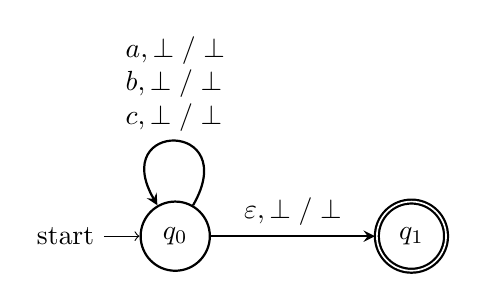
\begin{tikzpicture} [scale=1]
        \node[initial,thick,state] at (0,0) (q0) {$q_0$};
        \node[accepting,thick,state] at (3,0) (q1) {$q_1$};
        \path[->, thick, >=stealth]
        (q0) edge [loop,min distance = 1.25cm,above,in = 120, out = 60] 
        node[above,align=left] {$a,\perp/\perp$\\ $b,\perp/\perp$\\$c,\perp/\perp$} (q0)
        (q0) edge [above,in = -180, out = 0] 
        node[above,align=left] {$\varepsilon,\perp/\perp$} (q1)  
        ;
    \end{tikzpicture}
\end{center} 


\subsection*{$\left(b\right) \{a^mb^nc^q|m,n,p\geq0,mn=p\} $}
this is saimilarly with question 1.a. can be assume $\left(b\right)\Rightarrow\{aabbbcccccc\}=a^2b^3c^3\Rightarrow2*3=6$ that is condition with the question 
 and $u,v,w,x,y\in \left(b\right)\Rightarrow u=\{a\},~v=\{a\},~w=\{b\},~x=\{b\},y=\{bcccccc\}$\\
 At the first $v,x\neq \varepsilon\Rightarrow v=\{a\}\neq\varepsilon~and~x=\{b\}\neq\varepsilon$ that is true at this part.\\
 and then $|vwx|=3\leq2+3+6=11$ that is also available \\
 if we take i=3 that meaning $uv^iwx^iy=uv^3wx^3y=\{a aaa b bbb bcccccc\}$ the number of m=4,n=5,q=6 $4*5=20>6$.\\
 that meaning this set is not CFLs.\\\


\end{document}
